\documentclass[style=sailor,size=12pt]{powerdot}
\usepackage{epic,array,ecltree,url,calrsfs}
\usepackage[nointegrals]{wasysym}
\usepackage{listings}
\usepackage{epsfig}
\usepackage{amsmath}
\usepackage{amsfonts}
\usepackage{amssymb}
\usepackage{amsxtra}
\usepackage{amsthm}
\usepackage{mlextra} % Must be below ams packages
\usepackage{mathrsfs}
\usepackage{color}
\usepackage{array}
\usepackage{graphicx}
\graphicspath{ {../art/} }
\usepackage{bm}
\usepackage{tikz}
\usepackage{multicol}
\usepackage{enumitem}

\pdsetup{method=normal}
\title{Decision Procedures and \\ Computational Complexity}
\author{Foundations of Computer Science}
\date{\today}


\begin{document}
\maketitle
\begin{wideslide}[bm=,toc=]{Decision procedures vs semi-decision procedures}
\textbf{Decision Procedure:}
\begin{itemize}
\item<2-> A {\em decision procedure\/} for a set $A$ 
\begin{itemize}
\item<3-> returns ``yes'' on input $x$ {\bf iff} $x\in A$
\item<4-> returns ``no'' {\bf iff} $x\not\in A$
\end{itemize}
\item<5-> A decision procedure always says ``yes'' or ``no'' on any input.
\item<6-> Another term for decision procedure is ``algorithm''.
\end{itemize}
\pause[6]
\textbf{Semi-decision Procedure:}
\begin{itemize}
\item<8-> A {\em semi-decision\/} procedure for a set $A$ 
\begin{itemize}
\item<9-> returns ``yes'' on input $x$ {\bf iff} $x\in A$
\item<10-> returns ``no'' {\bf only if} $x\not\in A$
\end{itemize}
\item<11-> A semi-decision procedure need not terminate on an input $x$ if $x\not\in A$.
\end{itemize}
\end{wideslide}

% ADD slide from Ben Ari 2.5.1.

\begin{wideslide}[bm=,toc=]{Decidable vs undecidable problems}
\textbf{Decidable and Undecidable Sets:}
\begin{itemize}
\item<2-> A set is {\em decidable\/} iff there's a decision procedure for it.
\item<3-> Otherwise, it's called {\em undecidable}.
\end{itemize}
\pause[3]
\textbf{Semi-decidable Sets:}
\begin{itemize}
\item<5-> A set is {\em semi-decidable\/} iff there's a semi-decision procedure for it.
\item<6-> Decidable implies semi-decidable but the converse is not true. That is:
\begin{itemize}
\item<7-> All sets that are decidable are semi-decidable by definition,
\item<8-> \emph{but} there are semi-decidable sets that are undecidable.
\item<9-> Equivalently, the set of decidable sets is a proper subset of the set of
semi-decidable sets. 
\end{itemize}
\end{itemize}
\pause[6] \textbf{Application to Propositional Logic:}
\begin{itemize}
\item<11-> Both propositional satisfiability (PL-SAT) and propositional validity (PL-VAL) are decidable.
\end{itemize}
\end{wideslide}

\begin{wideslide}[bm=,toc=]{A Trivially Decidable Set}
\begin{itemize}
\item<1-> Let $S$ be the set of all even length strings over $\Sigma = \{0\}$. 
\item<2-> $S$ is decidable iff there is a decision procedure for $S$.
\item<3-> That is, if and only if there is an algorithm that takes a string $x \in
\Sigma^*$ and returns \emph{yes} if $x \in S$ and \emph{no} if $x \notin S$.
\item<4-> We have already seen a machine that does this: \pause[4]
\end{itemize}
\begin{figure}[h]
\centering
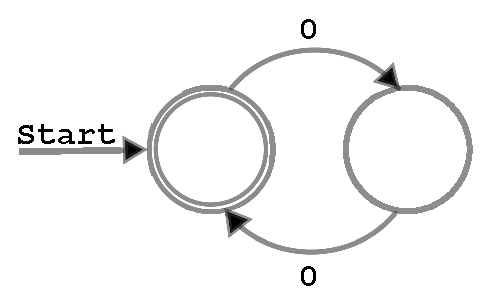
\includegraphics[width=2.5in, height=.75in,keepaspectratio=true]{evenzeroautomata.eps}
\label{2sp}
\end{figure}
\pause
To prove this is a decision procedure, you must show:
\begin{itemize}
\item<7-> It accepts all even length strings. 
\item<7-> It rejects all other strings. 
\item<7-> It always accepts or rejects (i.e.\ does not run forever).
\end{itemize}
\end{wideslide}

\begin{wideslide}[bm=,toc=]{The Halting Problem: an encounter with a 
  semi-decidable set}
\begin{itemize}
\item<1-> Let $M$ be a string that represents a well-formed computer program.
\begin{itemize}
\item<2-> That is, $M \in P$, where $P = \{M \in \Sigma^* | M \text{ is a well-formed 
  program}\}$.
\end{itemize}
\item<3-> Let $w \in \Sigma^*$ be a string that represents some input to the program.
\item<4-> Now let $(M,w)$ be a string that represents a pairing of a program and an
input, and define the language $H$ as follows: \pause[4]
\[H = \{(M,w) \in \Sigma^* | \text{ the program } M
\text{ eventually halts when run on input } w\}\]
\vspace{-5mm}
\item<6-> We can create a procedure that always says \emph{yes} when given a
string $(M,w) \in H$. 
\begin{itemize}
\item<7-> We use a universal Turing machine to simulate $M$ running on input $w$.
\item<8-> If $M$ halts, we return ``yes''
\end{itemize}
\item<9-> We can also create a procedure that will say \emph{no} \textbf{only} if $(M,w) \notin H$.
\item<10-> But there is no procedure that will \textbf{always} say \emph{no} if $(M,w) \notin H$
\end{itemize}
\end{wideslide}

\begin{wideslide}[bm=,toc=]{Decision Procedures in Propositional Logic}
\begin{defn}{2.40}[Ben Ari]
Let $\mathcal{U} \subseteq \mathcal{F}$ be a set of formulas. An algorithm
is a \emph{decision procedure} for $\mathcal{U}$ if given an arbitrary formula
$A \in \mathcal{F}$, it terminates and returns the answer \emph{yes} if
$A \in \mathcal{U}$ and the answer \emph{no} if $A \notin \mathcal{U}$.
\end{defn}
\begin{itemize}
\item Let $\mathcal{U}$ be the set of satisfiable formulas. Then a decision
procedure for $\mathcal{U}$ is called a decision procedure for satisfiability.
\item Similarly, if $\mathcal{U}$ is the set of valid formulas, a decision
procedure for $\mathcal{U}$ is a decision procedure for validity. 
\end{itemize} 
\end{wideslide}

\begin{wideslide}[bm=,toc=]{Refutation Procedures}
Recall \textbf{Theorem 2.39}: 
\begin{itemize}
\item $A$ is valid if and only if $\ngg A$ is unsatisfiable.
\item $A$ is satisfiable if and only if $\ngg A$ is falsifiable.
\end{itemize}

~\\
Therefore, a decision procedure for satisfiability can be used to decide validity: 
\begin{itemize}
\item To decide if $A$ is valid, apply decision procedure for satisfiability to $\ngg A$. 
\item This type of decision procedure is called a ``refutation procedure.'' 
\item Can be more efficient---only need to find a single counterexample.
\end{itemize} 
\end{wideslide}

\begin{wideslide}[bm=,toc=]{Examples of Decision Procedures for Satisfiability
  of Formulas in Propositional Logic}
\textbf{``Brute force'' approach:}
\begin{itemize}
\item Enumerate the truth table (requires $2^n$ entries for $n$ literals).
\end{itemize} 
\textbf{More efficient alternatives:}
\begin{itemize}
\item Resolution procedure / propositional resolution.
\item Davis--Putnam--Logemann--Loveland (DPLL) algorithm (also gives a model if
    the formula is satisfiable).
\end{itemize} 
\textbf{Note:} Both resolution and DPLL are ``nondeterministic'' (explanation
    of this term will follow shortly).
\end{wideslide}

\begin{wideslide}[bm=,toc=]{Measuring Complexity}
We measure the difficulty of a problem by the resources (time and space)
  required to solve it (with respect to some computational model).
\begin{itemize}
\item The time and space used are measured against input size.
\item A Turing Machine is the most commonly used model. 
\end{itemize}
\begin{defn}{}[Hopcroft et al]
A Turing Machine $M$ is said to be of \emph{time complexity} $T(n)$ [or to have
``running time $T(n)$''] if whenever $M$ is given an input $w$ of length
$n$, $M$ halts after making at most $T(n)$ moves...
\end{defn}
\begin{itemize}
\item Ex: if $T(n) = kn$ for some constant $k$, the problem is solvable in
\emph{linear} time.
\item Ex: if $T(n) = an^k + bn^{k-1}... + c$ the algorithm is solvable in polynomial
time.
\end{itemize}
\end{wideslide}

\begin{wideslide}[bm=,toc=]{Intuition: deterministic vs nondeterministic}
{\bf Characteristic behavior:} 
\begin{itemize}
\item<2-> A deterministic machine makes one ``decision'' at a time.
\item<3-> A non-deterministic machine makes all possible decisions at the same a time.
\end{itemize}
\pause[3]
{\bf Example:} consider a program designed to navigate a maze. 
\begin{itemize}
\item<5-> {\bf Deterministic behavior:} 
\begin{itemize}
\item<6-> When it reaches a fork, it must choose a single direction to explore.
\item<7-> Later, it can come back and try other directions. 
\item<8-> However, it can only test one at a time.
\end{itemize}
\item<9-> {\bf Nondeterministic behavior:}
\begin{itemize}
\item<10-> Whenever a nondeterministic program reaches a fork, it can explore all
directions at the same time, as if making copies of itself. 
\item<11-> The copy that finds the exit of the maze returns the answer.
\item<12-> The other copies die off. 
\item<13-> The effect is as though the machine always guesses the best choice.
\end{itemize}
\end{itemize}

\end{wideslide}

\begin{wideslide}[bm=,toc=]{$\id{P}$ and $\id{NP}$}
{\bf Complexity Classes ``$\id{P}$'' and ``$\id{NP}$''}
\begin{itemize}
\item $\id{P}$ and $\id{NP}$ are classes of problems (i.e. languages).
\item $\id{P}$ stands for ``polynomial'' and $\id{NP}$ stands for ``nondeterministic
polynomial.''
\end{itemize}
\pause
\begin{defn}{}[Hopcroft et al]
We say a language $L$ is in class $\id{P}$ if there is some polynomial $T(n)$ such
that $L = L(M)$ for some deterministic $\mli{TM}$ $M$ of time complexity
$T(n)$. 
\end{defn}

\pause
\begin{defn}{}[Hopcroft et al]
A language $L$ is in the class $\id{NP}$ (nondeterministic polynomial) if there
is a nondeterministic $\mli{TM}$ $M$ and a polynomial time complexity $T(n)$
such that $L = L(M)$, and when $M$ is given an input of length $n$, there are
no sequences of more than $T(n)$ moves of $M$.
\end{defn}
Observe that the above definitions imply $\id{P} \subseteq \id{NP}$.
\end{wideslide}

\begin{wideslide}[bm=,toc=]{$\id{NP}$ and $\id{coNP}$}
{\bf Complexity Classes ``$\id{NP}$'' and ``$\id{coNP}$''}
\begin{itemize}
\item $\id{coNP}$ is the complement of the class $\id{NP}$.
\end{itemize}

{\bf Examples:} Satisfiability ($\id{SAT}$) and Unsatisfiability ($\id{UNSAT}$) 
\begin{itemize}
\item<2-> What is the complexity of $\id{SAT}$ for Propositional Logic?
\begin{itemize}
\item<3-> Consider $(p\vee\neg q)\wedge(\neg p\vee q)$.
\item<3-> It is satisfiable ($p=q=T$ or $p=q=F$).
\item<3-> A nondeterministic algorithm can {\em guess\/} an interpretation and then {\em verify\/}
it satisfies the formula in time linear in the formula's length.
\item<3-> Guessing takes time linear in the number of propositional variables.
\item<3-> Hence it's possible to decide satisfiability of any propositional formula {\em nondeterministically\/}
in time proportional to its length.
\item<4-> Hence $\id{PL-SAT}$ belongs to $\id{NP}$, the class of problems 
solvable in Nondeterministic Polynomial time.
\end{itemize}
\end{itemize}
\end{wideslide}

\begin{wideslide}[bm=,toc=]{$\id{NP}$ and $\id{coNP}$ (continued)}
{\bf Complexity Classes ``$\id{NP}$'' and ``$\id{coNP}$''}
\begin{itemize}
\item $\id{coNP}$ is the complement of the class $\id{NP}$.
\end{itemize}
{\bf Examples:} Satisfiability ($\id{SAT}$) and Unsatisfiability ($\id{UNSAT}$) 
\begin{itemize}
\item<2-> What is the complexity of $\id{UNSAT}$ for Propositional Logic?
\begin{itemize}
\item<3-> If a formula is not satisfiable, it is unsatisfiable.
\item<3-> Thus, if $\mathcal{F}$ is the set of formulas in propositional logic
\pause[3]
  \[
    \mathcal{F} - \id{PL-SAT} = \id{PL-UNSAT}
  \]
  \vspace{-5mm}
\item<5->  $\id{PL-UNSAT}$ is in $\id{coNP}$ (not in $\id{NP}$ unless
    $\id{NP}=\id{coNP}$).
\end{itemize}
\end{itemize}
\end{wideslide}



\begin{wideslide}[bm=,toc=]{$\id{NP}$-hard and $\id{NP}$-complete}
\begin{itemize}
\item The following three statements are equivalent: 
\begin{itemize}
\item $\id{NP}$ contains problems with no deterministic polynomial time
solution.
\item There are problems in $\id{NP}$ that are \emph{not} in $\id{P}$.
\item $\id{P} \neq  \id{NP}$
\end{itemize}
\item Though widely conjectured, the above statements remain unproven.
\end{itemize}
\textbf{$\id{NP}$-hard and $\id{NP}$-complete}
\begin{itemize}
\item A problem is ``$\id{NP}$-hard'' if it is at least as hard as
every problem in $\id{NP}$.
\item A problem is ``$\id{NP}$-complete'' if it is \textbf{both} in $\id{NP}$ \textbf{and} $\id{NP}$-hard.
\item If any $\id{NP}$-complete problem can be solved in deterministic
polynomial time, this would imply that {\em every\/}
problem in $\id{NP}$ can be solved in deterministic polynomial time.
\begin{itemize}
\item In other words, this would prove $\id{P} = \id{NP}$
\end{itemize}
\end{itemize}
\end{wideslide}

\begin{wideslide}[bm=,toc=]{Two Alternative Possibilities for Relating Algorithm
  Classes P, NP, NP-Complete and NP-Hard}

\begin{figure}[h]
\centering
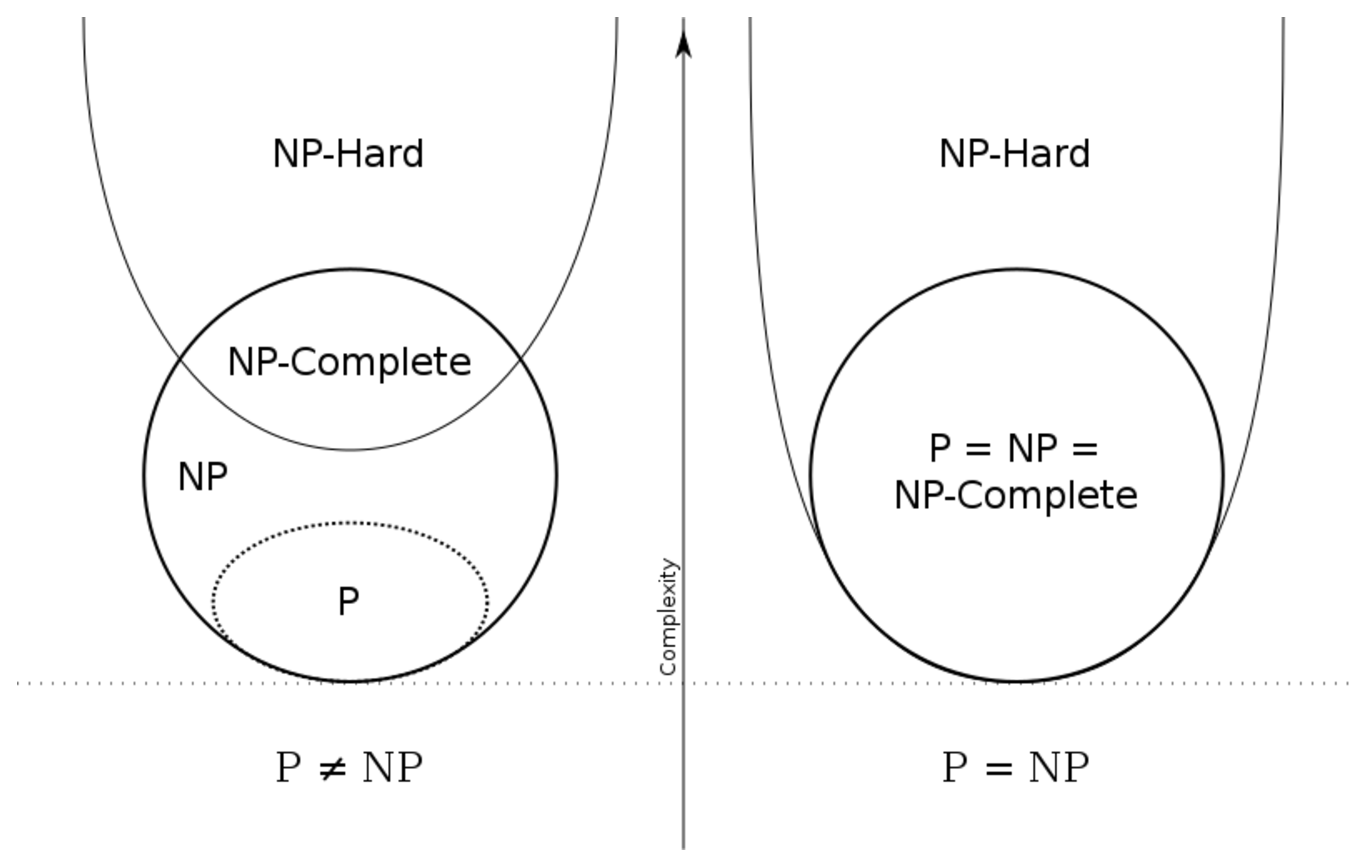
\includegraphics[width=4in, height=4in,keepaspectratio=true]{np_np-complete_np-hard.eps}
\label{2sp}
\end{figure}
By Behnam Esfahbod, CC BY-SA 3.0, \url{https://commons.wikimedia.org/w/index.php?curid=3532181}
\end{wideslide}

\begin{wideslide}[bm=,toc=]{Intuition for Reduction}
We say a problem $A$ \emph{reduces} to another problem $B$ if any algorithm that
solves problem $B$ can also be used to solve problem $A$.
\begin{itemize}
\item That is, solving $B$ is sufficient to solve both $A$ and $B$.
\item Informally, solving $B$ must be at least as hard as $A$, or harder.
\item Notation: $A$ reduces to $B$ is written $A \leq B$.
\end{itemize}
Note this definition implies that a problem generally \emph{reduces} to a
\emph{harder} problem, in contrast to what you might expect the word
\emph{reduce} to mean.
\\~\\
More formally: 
\vspace{-2ex}
\begin{defn}{}[\url{https://en.wikipedia.org/wiki/Many-one_reduction}]
Suppose $A$ and $B$ are formal languages over the alphabets $\Sigma$ and $\Gamma$, 
respectively. A many-one reduction from $A$ to $B$ is a total computable function 
$f : \Sigma^* \to \Gamma^*$ that has the property that each word $w$ is in $A$ if and only 
if $f(w)$ is in $B$ (that is, $A=f^{-1}(B)$).
\end{defn}
\end{wideslide}

\begin{wideslide}[bm=,toc=]{$\id{PL-SAT}$ and $\id{PL-VAL}$: $\id{NP-}$ and
  $\id{coNP-}$completeness}
\begin{itemize}
\item $\id{PL-SAT}$ is $\id{NP-}$complete (proofs due to Cook and Levin).
\item The complement of an $\id{NP-}$complete problem is $\id{coNP-}$complete.
\item Hence $\id{PL-UNSAT}$ is $\id{coNP-}$complete.
\item $\id{PL-UNSAT}$ many-one reduces to $\id{PL-VAL}$ in polynomial time.
\item Hence $\id{PL-VAL}$ is $\id{coNP-}$hard.
\item $\id{PL-INVAL}$ (find a falsifying interpretation) is in $\id{NP}$ and therefore $\id{PL-VAL}$ is in $\id{coNP}$.
\item Thus $\id{PL-VAL}$ is $\id{coNP-}$complete.
\item $\id{PL-VAL}$ is ``harder'' than $\id{PL-SAT}$; not in $\id{NP}$ unless $\id{NP} = \id{coNP}$ which is unlikely.
\item Things change in First Order Logic: $\id{FOL-SAT}$ becomes harder than $\id{FOL-VAL}$!
\end{itemize}
\end{wideslide}

\end{document}
